\chapter{Neural Networks} 


\label{Chapter2}

Neural networks also known as \ac{ANN} are machine learning algorithms that form the basis of deep learning. They inherit name and structure from neurons in the brain. Biological neurons transmit signals to one another through complex networks. This interconnected networking is realized though various architectures by \ac{ANN}s. Sets of artificial neurons are stacked on top of each other to form a layer. A typical neural network consists of many such layers that are connected to each other. The first layer is called input layer, the final layer is termed output layer and the layers in-between are called hidden layers. A neural network with three hidden layers is depicted in Fig~\ref{fig:nn}. The transmission of data across the nodes or artificial neurons happens through the connections. Each and every node has a specific weight and threshold associated. The output from a node is passed through the connection only if the value is above the threshold. Neural network approaches are data-driven. Their performance improves as they learn through training on a dataset. 

\begin{figure}
	\centering
\begin{neuralnetwork}[height=5]
	\newcommand{\x}[2]{$x_#2$}
	\newcommand{\y}[2]{$\hat{y}_#2$}
	\newcommand{\hfirst}[2]{\small $h^{(1)}_#2$}
	\newcommand{\hsecond}[2]{\small $h^{(2)}_#2$}
	\inputlayer[count=4, bias=true, title=Input\\layer, text=\x]
	\hiddenlayer[count=5, bias=false, title=Hidden\\layer 1, text=\hfirst] \linklayers
	\hiddenlayer[count=4, bias=false, title=Hidden\\layer 2, text=\hsecond] \linklayers
	\hiddenlayer[count=3, bias=false, title=Hidden\\layer 3, text=\hsecond] \linklayers
	\outputlayer[count=2, title=Output\\layer, text=\y] \linklayers
\end{neuralnetwork}
\caption{Depiction of a neural network with an input layer, three hidden layers and an output layer}\label{fig:nn}
\end{figure}


To further understand the working of a neural network, we can imagine each node to be solving the problem of linear regression. For example consider a node with four inputs ($x_i, i=1,2,\dots4$), four weights ($w_i, i=1,2,\dots4$) and a bias:

\begin{equation}
\sum_{i=1}^{m} w_{i} x_{i}+\text { bias }=w_{1} x_{1}+w_{2} x_{2}+w_{3} x_{3}+w_{4} x_{4}+\text { bias }
\end{equation}

The output of the node is the above summation after going through an activation function $a$:
\begin{equation}
\text { output }=a(x)=\left\{\begin{array}{l}
1 \text { if } \sum w_{1} x_{1}+b \geq 0 \\
0 \text { if } \sum w_{1} x_{1}+b<0
\end{array}\right.
\end{equation}
In the above example, the given activation function of this node propagates the value $1$ only when the weighted sum of it's inputs is non-negative. When the condition of an activation function are met the output of this node becomes an input to the node to which it's connected. Due to the process of forwarding values through a network, an \ac{ANN} is also called feed-forward network. Complex networks with multiple layers of these nodes are used in practical tasks. An important category of machine learning task is supervised learning. It involves training a neural network on labeled datasets. The goal of training a neural network is to minimize a cost function that enforces the closeness of predicted and real output labels. During the training the network reorganizes it's weights based on the loss function. This process of updating weights is called optimization. Each update is aimed at reaching a minimum of the loss function. A popular optimization method is gradient descent. It guides the model in the direction of reducing errors to reach an optima. The development of back-propagation (\cite{rumelhart1986learning}) has been instrumental in successful implementation of optimization algorithms for neural networks.  


\subsection{Convolutional Neural Networks}

The neural network depicted in \ref{fig:nn} is an example of densely connected network, where all the neighboring nodes are connected with one another. As the size of data increases (say large image data), and the network becomes more complex, the number of parameters increases exponentially. To address this and also to be more suitable for image data \ac{CNN}s were formulated. \ac{CNN}s are extensively used in computer vision tasks like image classification, object detection, image segmentation (\cite{voulodimos2018deep}). The three main building blocks of a \ac{CNN} are Convolution, Activation and Pooling. Each of these layers are discussed below:

\subsection{Convolution}

Images are digitally stored in the form of 2D or 3D matrices depending on the format. A convolution kernel (also known as filter) is a matrix that operates on these images and transforms them based on the kernel values. These kernel values are also known as weights in the neural network terminology. Typically, the size of the kernel is much smaller than that of the image. Many sets of these kernels form the convolution layer of the \ac{CNN}.  The movement of the kernel over the image can be made either by a single pixel or multiple pixels. This step size is called stride ($s$). The resulting output of a convolution between filter and image is called a feature map. Consider a kernel $h$ and input image $f$ with $m$ rows and $n$ columns. Convolution between $h$ and $f$ results in a feature map $g$: 
\begin{equation}
g[m, n]=(h * f)[m, n]=\sum_{i} \sum_{j} h[i, j] f[m-i, n-j]
\end{equation}

\begin{figure}[!htbp]
	\centering
	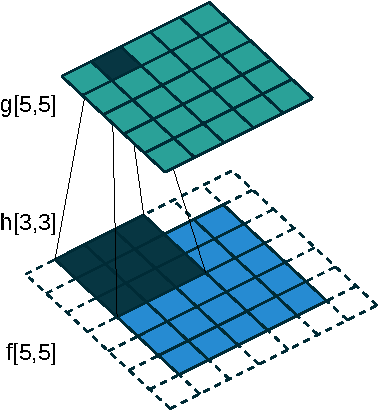
\includegraphics[width=0.4\linewidth]{./Figures/convol-crop.pdf}
	\caption{Convolution of an input image of dimensions 5$\times$5 with a filter of dimensions 3$\times$3.(\cite{dumoulin2016guide})}
	\label{fig:conv}
\end{figure}

Given in Fig~\ref{fig:conv} is a representation of the convolution operation. Zero padding is used to manipulate the dimensions of the feature maps. In the above Figure above it is indicated with dotted lines. The function of padding here is to maintain same dimensions in the input image $f$ and the feature map $g$. A \ac{CNN} learns features from the input through many convolutional layers. The earlier layers learn general features like edges, contrast, the deep layers learn more abstract and finer details.  

\subsection{Activation Layer}

The activation layer that follows the convolution layer in a \ac{CNN} is most commonly the \ac{ReLU} activation function, depicted in Fig~\ref{fig:relu}.

\begin{figure}[!htbp]
	\centering
	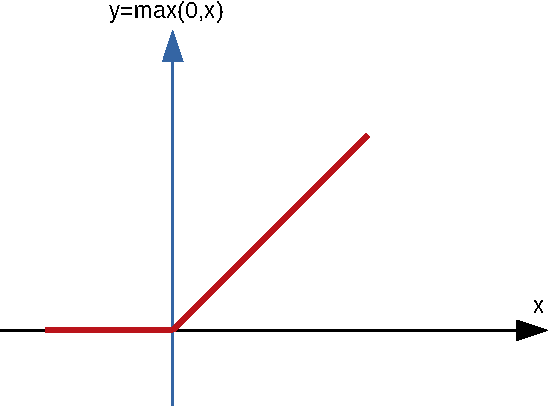
\includegraphics[width=0.6\linewidth]{relu-crop.pdf}
	\caption{The \ac{ReLU} function}
	\label{fig:relu}
\end{figure}


Many of the task based on images are non-linear in nature. Whether a computer vision task like identifying objects in an image or a medical imaging task involving tumor detection, the relationships are far from being linear. The \ac{ReLU} function increases this required non-linearity in the \ac{CNN}. 

\subsection{Pooling Layer}

The third building block of a \ac{CNN} is the pooling layer. Pooling operation is mainly used to reduce the dimensions of a tensor which enables faster computation. Max pooling is the most commonly used pooling operation. A max pooling operator of a particular size returns the maximum value of a selected region in the feature map. Similar to a filter it is implemented with a specific stride. A max pooling filter with $s=2$ is depicted in Fig~\ref{fig:mp}.

\begin{figure}[!htbp]
	\centering
	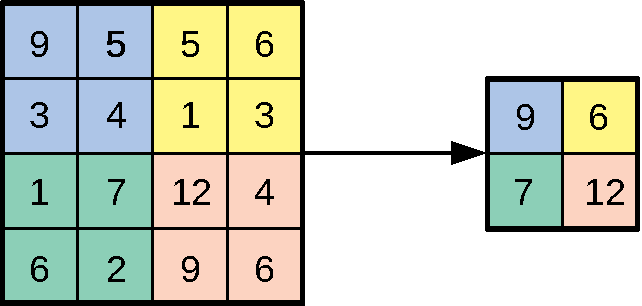
\includegraphics[width=0.6\linewidth]{maxP-crop.pdf}
	\caption{Max pooling with 2$\times$2 filter and stride 1}
	\label{fig:mp}
\end{figure}


A \ac{CNN} with $2$ convolutional layers, $2$ activation layers and $2$ pooling layers is represented in Fig~\ref{fig:trad_cnn}. Layer number is given by $l$. The first and the last layer are the input and output respectively. Usually the last set of layers in a \ac{CNN} used for classification, regression tasks is a fully-connected layer which is similar to the neural network represented in Fig~\ref{fig:nn}. With the advent of powerful computation tools and efficient parallel processing, neural networks with many layers could be implemented. The term deep learning was coined for networks with this "deep" design (\cite{lecun2015deep}). Deep neural networks could be trained over large datasets and they outperformed many existing state of the art algorithms in computer vision. In this thesis we focus specifically on \ac{CNN}s under the umbrella of deep neural networks.  




\begin{figure}[t!]
	\centering
	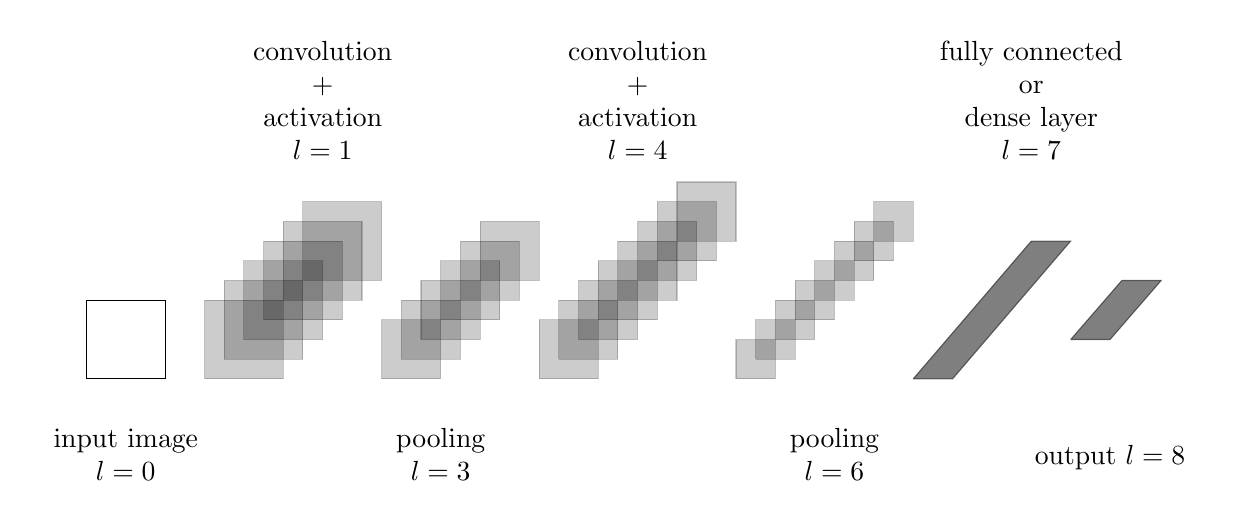
\begin{tikzpicture}
	\node at (0.5,-1){\begin{tabular}{c}input image\\ $l = 0$\end{tabular}};
	
	\draw (0,0) -- (1,0) -- (1,1) -- (0,1) -- (0,0);
	
	\node at (3,3.5){\begin{tabular}{c}convolution \\+\\ activation\\ $l = 1$\end{tabular}};
	
	\draw[fill=black,opacity=0.2,draw=black] (2.75,1.25) -- (3.75,1.25) -- (3.75,2.25) -- (2.75,2.25) -- (2.75,1.25);
	\draw[fill=black,opacity=0.2,draw=black] (2.5,1) -- (3.5,1) -- (3.5,2) -- (2.5,2) -- (2.5,1);
	\draw[fill=black,opacity=0.2,draw=black] (2.25,0.75) -- (3.25,0.75) -- (3.25,1.75) -- (2.25,1.75) -- (2.25,0.75);
	\draw[fill=black,opacity=0.2,draw=black] (2,0.5) -- (3,0.5) -- (3,1.5) -- (2,1.5) -- (2,0.5);
	\draw[fill=black,opacity=0.2,draw=black] (1.75,0.25) -- (2.75,0.25) -- (2.75,1.25) -- (1.75,1.25) -- (1.75,0.25);
	\draw[fill=black,opacity=0.2,draw=black] (1.5,0) -- (2.5,0) -- (2.5,1) -- (1.5,1) -- (1.5,0);
	
	\node at (4.5,-1){\begin{tabular}{c}pooling \\ $l = 3$\end{tabular}};
	
	\draw[fill=black,opacity=0.2,draw=black] (5,1.25) -- (5.75,1.25) -- (5.75,2) -- (5,2) -- (5,1.25);
	\draw[fill=black,opacity=0.2,draw=black] (4.75,1) -- (5.5,1) -- (5.5,1.75) -- (4.75,1.75) -- (4.75,1);
	\draw[fill=black,opacity=0.2,draw=black] (4.5,0.75) -- (5.25,0.75) -- (5.25,1.5) -- (4.5,1.5) -- (4.5,0.75);
	\draw[fill=black,opacity=0.2,draw=black] (4.25,0.5) -- (5,0.5) -- (5,1.25) -- (4.25,1.25) -- (4.25,0.5);
	\draw[fill=black,opacity=0.2,draw=black] (4,0.25) -- (4.75,0.25) -- (4.75,1) -- (4,1) -- (4,0.25);
	\draw[fill=black,opacity=0.2,draw=black] (3.75,0) -- (4.5,0) -- (4.5,0.75) -- (3.75,0.75) -- (3.75,0);
	
	\node at (7,3.5){\begin{tabular}{c}convolution \\+\\ activation\\ $l = 4$\end{tabular}};
	
	\draw[fill=black,opacity=0.2,draw=black] (7.5,1.75) -- (8.25,1.75) -- (8.25,2.5) -- (7.5,2.5) -- (7.5,1.75);
	\draw[fill=black,opacity=0.2,draw=black] (7.25,1.5) -- (8,1.5) -- (8,2.25) -- (7.25,2.25) -- (7.25,1.5);
	\draw[fill=black,opacity=0.2,draw=black] (7,1.25) -- (7.75,1.25) -- (7.75,2) -- (7,2) -- (7,1.25);
	\draw[fill=black,opacity=0.2,draw=black] (6.75,1) -- (7.5,1) -- (7.5,1.75) -- (6.75,1.75) -- (6.75,1);
	\draw[fill=black,opacity=0.2,draw=black] (6.5,0.75) -- (7.25,0.75) -- (7.25,1.5) -- (6.5,1.5) -- (6.5,0.75);
	\draw[fill=black,opacity=0.2,draw=black] (6.25,0.5) -- (7,0.5) -- (7,1.25) -- (6.25,1.25) -- (6.25,0.5);
	\draw[fill=black,opacity=0.2,draw=black] (6,0.25) -- (6.75,0.25) -- (6.75,1) -- (6,1) -- (6,0.25);
	\draw[fill=black,opacity=0.2,draw=black] (5.75,0) -- (6.5,0) -- (6.5,0.75) -- (5.75,0.75) -- (5.75,0);
	
	\node at (9.5,-1){\begin{tabular}{c}pooling\\ $l = 6$\end{tabular}};
	
	\draw[fill=black,opacity=0.2,draw=black] (10,1.75) -- (10.5,1.75) -- (10.5,2.25) -- (10,2.25) -- (10,1.75);
	\draw[fill=black,opacity=0.2,draw=black] (9.75,1.5) -- (10.25,1.5) -- (10.25,2) -- (9.75,2) -- (9.75,1.5);
	\draw[fill=black,opacity=0.2,draw=black] (9.5,1.25) -- (10,1.25) -- (10,1.75) -- (9.5,1.75) -- (9.5,1.25);
	\draw[fill=black,opacity=0.2,draw=black] (9.25,1) -- (9.75,1) -- (9.75,1.5) -- (9.25,1.5) -- (9.25,1);
	\draw[fill=black,opacity=0.2,draw=black] (9,0.75) -- (9.5,0.75) -- (9.5,1.25) -- (9,1.25) -- (9,0.75);
	\draw[fill=black,opacity=0.2,draw=black] (8.75,0.5) -- (9.25,0.5) -- (9.25,1) -- (8.75,1) -- (8.75,0.5);
	\draw[fill=black,opacity=0.2,draw=black] (8.5,0.25) -- (9,0.25) -- (9,0.75) -- (8.5,0.75) -- (8.5,0.25);
	\draw[fill=black,opacity=0.2,draw=black] (8.25,0) -- (8.75,0) -- (8.75,0.5) -- (8.25,0.5) -- (8.25,0);
	
	\node at (12,3.5){\begin{tabular}{c}fully connected\\ or\\ dense layer\\$l = 7$\end{tabular}};
	
	\draw[fill=black,draw=black,opacity=0.5] (10.5,0) -- (11,0) -- (12.5,1.75) -- (12,1.75) -- (10.5,0);
	
	\node at (13,-1){\begin{tabular}{c}output $l = 8$\end{tabular}};
	
	\draw[fill=black,draw=black,opacity=0.5] (12.5,0.5) -- (13,0.5) -- (13.65,1.25) -- (13.15,1.25) -- (12.5,0.5);
	\end{tikzpicture}
	\caption{Architecture of a typical \ac{CNN}. This representation was first proposed by \cite{lecun1995convolutional}.}
	\label{fig:trad_cnn}
\end{figure}

\subsection{Neural Networks for Image Reconstruction}

Image to image translation tasks require the \ac{CNN} to map from image in one domain to an image in another related domain. This requires the design of the \ac{CNN} to be quite different from the one depicted in Fig~\ref{fig:trad_cnn}. Convolution and pooling operations compress the input to obtain an abstract representation in lower dimensions. To transform the output into an image from the lower dimensional representation, transposed convolution operators are used. In contrast to the compressing nature of convolutions, they expand the input feature map. The combination of convolution+pooling and transposed convolutions are adjusted depending on the dimensions of the input and output images. Transposed convolution is shown in Fig~\ref{fig:tc}. Essentially the transposed convolution spatially reverses the dimensions of the convolution+pooling operation. 

\begin{figure}[!htbp]
	\centering
	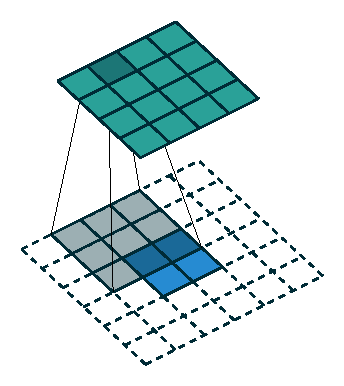
\includegraphics[width=0.5\linewidth]{transposed.pdf}
	\caption{Transposed convolution over a $2\times2$ input to get a $4\times4$ output. (\cite{dumoulin2016guide})}
	\label{fig:tc}
\end{figure}

Transposed convolutions are used in many tasks like super resolution, image segmentation, denoising and image reconstruction. This version of \ac{CNN} appropriate for image reconstruction is represented in Fig~\ref{fig:fcn}

\begin{figure}[!htbp]
	\centering
	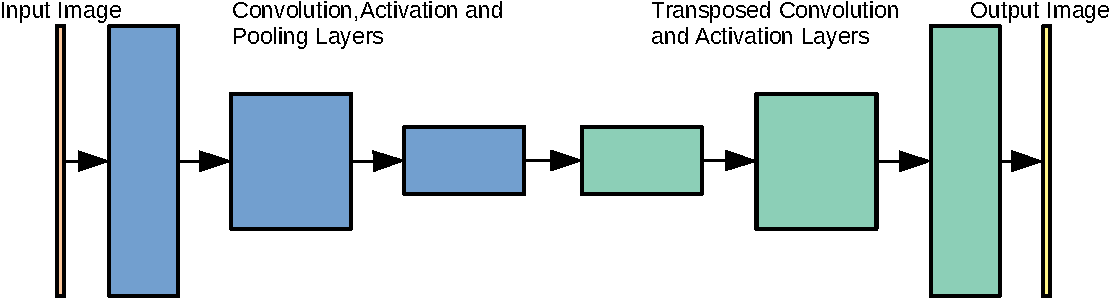
\includegraphics[width=1.0\linewidth]{fcn-crop.pdf}
	\caption{\ac{CNN} for image to image translation tasks. This example has an identical structure in convolution path and the transposed convolution path.}
	\label{fig:fcn}
\end{figure}

These architectures are sometimes referred to as \ac{CED}, since they contain two distinct paths of down sampling of input and up sampling of lower dimensional representation. The building blocks described in this section essentially form the basis of \ac{CNN}s proposed in this thesis. The next chapter consists of a review of existing works in deep learning applied to medical image reconstruction. And the following chapters describe the proposed methods. 



